\chapter{Testing}
Testing is important and integral part of any software development project. It is necessary to carry out testing throughout the implementation, as well as once the system is completed, in order to make sure the software developed functions correctly according to the requirements and the design.
%The disruption engine consists of a number of individual components and algorithms.These are tested using a number of unit tests. Due to the nature of the engine, stress tests were carried out to test it for any memory leaks and performance issues. Evaluation of the output of the disruption engine will be performed by first carrying out further literature review to find some guidance on what window for the data to consider to use and what weights to use for optimal results. This will be followed by running the system on a given set of data (e.g. a week worth of AVL data) and comparing the output with the actual state of the network during this period.

%The user interface consists of a simple web application capable of displaying list of disruptions. Testing and evaluation of this web application will be performed as user testing. As I mentioned above, some feedback and problems were identified which will be addressed and fixed. Follow up user tests will be carried out by giving access to friends and family to the web site to use and give feedback on. This should give reasonable confidence in the correctness of the user interface as there is no complex logic incorporated in the web front end application.
\section{Unit Testing} 
As described in the previous chapters, the system is composed of a number of classes, each of them representing different part of the bus network with its own functionalities and responsibilities. Throughout the development of the product a number of unit tests have been carried out in order to ensure that each of the classes functions correctly as per requirements, and carries out the required task. Each module was tested separately before being connected to the rest of the system.

\section{White Box Testing}
Apart from the unit testing through the development of the system, I have also made great use of the debugging tool provided by IntelliJ IDEA\footnote{https://www.jetbrains.com/idea/} integrated development environment (IDE). This was the main IDE used for the development of this project (both the disruption engine and the user interface web application) and has provided many useful tools and support. The built-in debugger allowed me to carry out inspection of the code during its execution while still developing the application, in order to make sure that desired outcome is produced. The debugging tool allows us to halt the execution (in real time) at specific point during the calculations and examine the state of the program (the values of all variables). This has proved very useful as it allowed me to quickly fix and rectify any issues early in the implementation, which otherwise could have remained hidden.

\section{Functional Testing}
Functional testing is form of black box testing. It is called black box, because we test the software product by feeding it some input and examining the generated output without having knowledge internal states of the software. Functional testing does not mean we are carrying out tests on individual methods/functions or classes/components, it means that we are testing parts of the functionalities stated in the requirements. Since the proposed system consists of two sub-systems I was able to perform separate functional testing of each of the systems.

The disruption engine was tested by having semi-automated functional tests which feed the system with a feed file and then examine the produced results. Some of the example test cases include:
\begin{itemize}
	\item Correct, but empty feed file is pushed to the system.
	\item Single correct feed file is pushed, containing a single bus reading.
	\item Two correct feed files are pushed, each containing a single reading from the same bus.
	\item A malformed feed file is pushed to the system.
	\item A batch of feed files is pushed to the system.
\end{itemize}

The web application part of the system does not contain much complex logic. The most complicated part is retrieving the right data. This required some more complex SQL queries which were tested manually using pgAdmin\footnote{\url{http://www.pgadmin.org/}} as a SQL editor program. However, the rest of the functionalities of the user interface have been tested by me throughout the implementation. As the user interface is basically visualising the generated output from the disruption engine, two main scenarios have been considered during its testing. The first is testing the functionalities while the disruption engine is either not running or it does not produce any output. The other test is performed while new output is being generated by the back end (disruption engine) and the user interface is continuously updating itself. In addition to these scenarios, due to the fact the system distinguishes between three types of user roles, I have assumed each one of them and carried out manual tests to verify the correct behaviour of the system. 

Some feedback has been received regarding the user interface during demonstration and discussions with CentreComm and my supervisor. All remarks and suggestions from the received feedback have been addressed. In addition to that I have asked family and friends to spend time and test the functionality of the user interface. For this I provided them with a list of use cases and the respective expected behaviour. This has proved useful in identifying some issues with the functionality and the compatibility of the product with different web browsers and systems. All of the identified problems have been addressed and rectified following the received feedback.

%USER INTERFACE - this consistes of testing the user interface in live state (while the engine was generating more input and updating the state) and also at paused state when the engine did not run or did not generate any input. I considered all three user roles and tested the system for the expected output.

%This was carried out by manually testing the functionality of the web application and verifying that it resulted in the correct output. The user interface has been tested by me throughout development, some feedback has been received on it during demonstration and discussions with CentreComm and my supervisor. In addition to that I have asked family and friends to spend time and test the functionality of the user interface for this I provided them with a list of use cases and the expected behaviour. This has proved useful in identifying some issues with the functionality and the compatibility of the product with different web browsers and systems. All of the identified problems have been addressed and rectified after that.

\section{Stress Testing}
One of the main requirements for detecting the disruptions in the bus network is for it to be calculated in real time. Because of this I needed to make sure that the implementation is able to cope with large amounts of data quickly. Each bus reading that is received as part of the AVL feed files is on average $100$ bytes. There could be roughly up to $7000$ buses active in the bus network at each single point in time. This means that the system should be capable of processing $1$MB of data every $30$ seconds as close to real time as possible. Also, as the system will run continuously with more data being pushed to the system throughout its execution, it needs to be ensured that any memory that is occupied by irrelevant (old) data is discarded appropriately without causing any memory leaks. 

The approach that I have taken in order to test the system for such performance issues consisted of creating an automated script for simulating the feed pushing to the tool. This program takes two main input parameters. One is the directory in which the feeds for the simulation are being stored and the second main input is the rate at which these files are copied to the directory used by the disruption engine for monitoring. Currently, as discussed previously in this report, the AVL data files which were provided for this project are generated every 5 minutes. However, this could be changed in future if the tool goes into production. For this reason I need to make sure that the proposed prototype is capable of dealing with all of the data that is being pushed to the engine every 30 seconds (as this is the current rate iBus equipped buses transmit data). Apart from the rate at which new data is pushed to the tool, the performance of our system depends mainly on how much data is pushed (e.g. during the night hours there are less active buses thus less data generated compared to daytime) and also on how many disruptions are detected in the system. It is obvious that if there is more data to be processed, the system would naturally take longer. However, the second statement is because the system only updates the database information for a route, run and section only if there are changes. This means that the update time could vary greatly depending on the number of changes at each network update. In order to minimise the impact of this, the system is implemented in such a way that it makes all database updates (writes) as one single transaction, after the bus network representation is updated. This means that the main performance bottleneck of the system becomes the updating of the database. The initial versions of the prototype did not make use of a database, but rather wrote the output into flat CSV files. The reason for adding and using a database instead of CSV files is that it allows us more easily to analysis and query the state of the bus network in the past. Having a database with the historical information, enables us to write simple to complex SQL queries which to produce insightful reports, analysis and statistics. These are all features that have received a lot of positive feedback from TFL during presentations and demonstrations.

Simulations were run to make sure the system is capable of processing and updating itself as close as possible to real time. These tests have been carried out on a laptop running Intel Core i7-3610QM with 16GB DDR3 1600Mhz of ram and Windows 10 x64 bit operating system. The simulations consisted of feeding the tool with a week's worth of data that was provided by TFL. The data was made of 21629 separate (each one for a single bus operator) AVL feeds which have been group into 2814 batches according to their timestamps. The total size of the sample is 1.07 Gigabyte (1076394754 bytes) and the average size of a single feed file is 49.77 Kilobytes (49766.27 bytes). I ran a number of simulations with this data, keeping all parameters the same and re-initialising the system before each run. The only parameter I altered, to make sure the system is capable of handling data at higher rates, is the rate at which the feed simulation program pushed the AVL files. The results can be seen on figure~\ref{fig:stressTestResults} shown below. From the results, I can conclude that even on a normal computer in a development environment, the system is capable of producing output in almost real-time. The memory usage can also be seen in the results shown on figure~\ref{fig:stressTestResults} below. The memory was measured through the execution of the tool and readings were taken every minute. The memory usage is highly dependent on the amount of the data being processed and also on when the Java Virtual Machine (JVM\footnote{http://www.oracle.com/webfolder/technetwork/tutorials/obe/java/gc01/index.html}) garbage collector executes. The latter is because the system might already have removed all references to some objects. However, this memory would not be unallocated until the JVM garbage collector is called.

The system current implementation is updating each route in the network consecutively. However, the system has been implemented with concurrent execution of this calculation in mind. This means that it could easily be updated such that each route is concurrently processed. This is also the case for the parsing of the CSV feed files and observation extraction. As the aim of this project is to built a prototype, I have decided not to spend the limited project time on such optimisations as it is more important to prove if this is viable solution. As it can be seen from the stress tests carried out even without such parallelism (multiple threads) in place, the system is capable of generating output in less than a second. This means that the bottleneck for achieving real-time updates to the users is the user interface implementation (e.g. how often the client web browser will poll the server for updates).

\begin{figure}[ht!]
	\makebox[\textwidth][c]{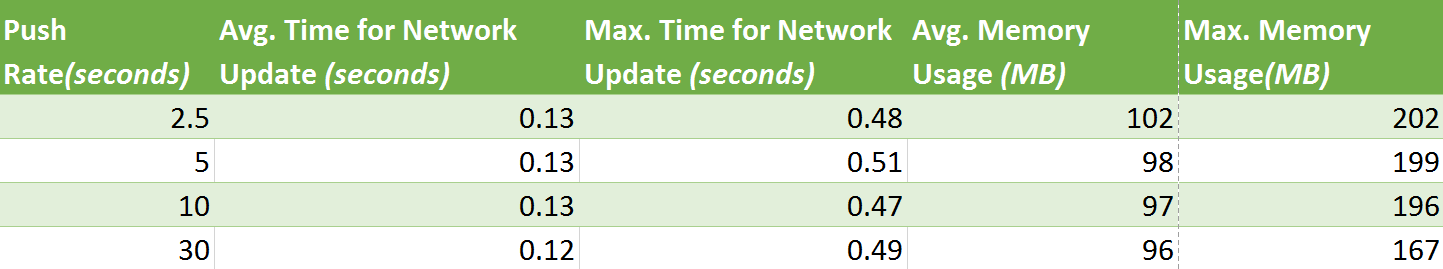
\includegraphics[width=1\textwidth]{Figures/StressTestResults.png}}
	\caption{Stress test results}
\label{fig:stressTestResults}
\end{figure}

%The results shows us that there are not problems with dealing with large amount of information in real time even on a normal mobile computer. It can also be seen that memory usage is within the capabilities of typical modern computer. We can see big variations in the memory usage, however this is normal as we do not explicitly allocate and deallocate memory. Scala runs on the Java Virtual Machine (JVM) which has garbage collector reponsible for freeing up unused memory. The only thing the programmer need to make sure for is that any objects that are unused should have no references pointing to them, then when JVM garbage collector executes it will return (free up) all unused memory. This means that our system memory usage depends on:
%\begin{itemize}
%	\item How fast new data is pushed.
%	\item How much data is being used (as discussed in the previous chapter).
%	\item How often the garbage collector executes.
%\end{itemize}